\section{Experiments}
\label{sec:experiments}

\subsection{Setup}
\label{sec:setup}

\paragraph{Benchmarks.} We evaluate on five diverse interactive environments:
\begin{itemize}
    \item \textbf{ALFWorld}~\citep{shridhar2021alfworld}: Text-based household tasks (pick-and-place, clean, heat, cool, examine, pick-two). We use the \texttt{eval\_out\_of\_distribution} split with 134 environments across 6 task types.
    \item \textbf{WebShop}~\citep{yao2022webshop}: E-commerce product search and purchase. Agents must find products matching natural language instructions by searching, browsing, selecting options, and buying. We evaluate on 100 sessions with 1,000 products. Success is measured by reward (0--1 scale based on attribute matching); we report both average reward and success rate (reward $\geq 0.5$).
    \item \textbf{ScienceWorld}~\citep{wang2022scienceworld}: Text-based science experiment simulation with 30 task types requiring multi-step scientific reasoning. For the formal no-gate comparison used in this paper, we follow the Step~4 runbook protocol: 111 test episodes spanning 12 core task types, with up to 10 test variations per task. We report both success rate and average raw score on the native ScienceWorld scale.
    \item \textbf{HotPotQA}~\citep{yang2018hotpotqa}: Multi-hop question answering over Wikipedia. Agents use Search, Lookup, and Finish actions to find and synthesize information across multiple articles. We evaluate on 500 randomly sampled validation examples and report exact match (EM) and F1 scores.
    \item \textbf{ToolBench}~\citep{qin2023toolllm}: API tool-use benchmark based on StableToolBench~\citep{guo2024stabletoolbench} with 765 solvable queries across 6 subsets (G1--G3). Agents call real-world API functions to answer user queries. We report pass rate (agent submits a non-empty answer via the Finish action).
\end{itemize}

\paragraph{Systems Compared.}
\begin{itemize}
    \item \textbf{ReAct Baseline}: Standard ReAct with few-shot prompting, no memory.
    \item \textbf{Reflexion}~\citep{shinn2023reflexion}: Episode-level self-reflection injected at the start of each retry. The agent runs two trials: the first trial collects failures, and the second trial benefits from reflections generated after the first. For the formal ScienceWorld Step~4 comparison, we report a corrected final metric that reuses pass~0 when pass~0 already solved the episode.
    \item \textbf{ExpeL}~\citep{zhao2024expel}: Cross-task insight extraction by comparing success and failure trajectories. After Epoch~1, abstract insight rules are extracted and injected at episode start in Epoch~2. We reproduce ExpeL on our same LLM backbone for fair comparison.
    \item \textbf{Offline memory (ScienceWorld only)}: A two-stage variant used in the Step~4 runbook. It first collects memory on the ScienceWorld train split without retrieval, then evaluates on the test split with in-loop retrieval enabled.
    \item \textbf{\method{}}: Our failure-triggered in-loop memory system. We report Epoch~1 (first pass, building memory) and Epoch~2 (with accumulated memory from Epoch~1).
\end{itemize}

\paragraph{Implementation.} For ALFWorld and WebShop, we use Qwen3.5-9B as the agent LLM, with the same model serving as the failure judge. DeepSeek-V3.2 is used as the memory extractor (ALFWorld/WebShop) and as the agent LLM for ScienceWorld, HotPotQA, and ToolBench (where the larger model is needed for complex reasoning). All LLMs are accessed via the SiliconFlow API. Sentence embeddings use all-MiniLM-L6-v2 running locally. Memory retrieval uses BM25 + embedding with RRF ($k=60$), returning top-3 entries. Maximum steps per episode: 50 (ALFWorld), 15 (WebShop), 8 (HotPotQA), and 12 (ToolBench). The formal ScienceWorld Step~4 protocol uses a dedicated 100-step limit; implicit judge-based failure detection is disabled and the system relies on explicit rules, so judge-token costs are not part of the reported ScienceWorld main results.

\subsection{Main Results}
\label{sec:main_results}

\begin{table}[t]
\centering
\caption{Main results on the four benchmarks that share the same multi-epoch evaluation protocol. 95\% bootstrap confidence intervals (10K resamples) are shown for success rates. Tok/env reports total token cost per environment across all passes (in thousands), including agent, judge, and extractor. Best results in \textbf{bold}. ScienceWorld uses a dedicated formal Step~4 no-gate protocol and is reported separately in Table~\ref{tab:sw_step4}.}
\label{tab:main_results}
\footnotesize
\setlength{\tabcolsep}{2.0pt}
\begin{tabular}{l cc ccc ccc cc}
\toprule
\multirow{2}{*}{System} & \multicolumn{2}{c}{ALFWorld} & \multicolumn{3}{c}{WebShop} & \multicolumn{3}{c}{HotPotQA} & \multicolumn{2}{c}{ToolBench} \\
\cmidrule(lr){2-3} \cmidrule(lr){4-6} \cmidrule(lr){7-9} \cmidrule(lr){10-11}
 & Succ. & Tok & Succ. & Rew. & Tok & EM & F1 & Tok & Pass & Tok \\
\midrule
Baseline & 91.0\tiny{[86,96]} & 52.9 & 38.0\tiny{[29,47]} & .38 & 38.3 & .40 & .50 & 5.5 & 62.8 & 6.3 \\
Reflexion & 94.0\tiny{[90,98]} & 53.8 & 45.0\tiny{[35,55]} & .41 & 41.8 & .44 & .53 & 6.1 & 81.4 & 5.6 \\
ExpeL & 94.8\tiny{[91,99]} & 50.8 & \textbf{49.0}\tiny{[39,59]} & \textbf{.44} & 38.8 & \textbf{.44} & \textbf{.54} & 6.1 & \textbf{90.6} & 4.9 \\
\midrule
\method{} E1 & 91.8 & 56.4 & 40.0 & .39 & 46.0 & .40 & .49 & 7.2 & 62.1 & 7.7 \\
\method{} E2 & \textbf{95.5}\tiny{[92,99]} & 53.5 & 44.0\tiny{[34,54]} & .42 & 45.2 & .43 & .52 & 7.1 & 75.3 & 7.1 \\
\bottomrule
\end{tabular}
\vspace{0.3em}

{\footnotesize Tok = avg effective tokens (K) per task: for each task, we count the tokens from the epoch that produced its final result (E1 tokens for tasks solved in E1, E2 tokens for retried tasks), then average over all $N$ tasks. Reflexion/ExpeL report the final pass (Trial~1 / Epoch~2).}
\end{table}

Table~\ref{tab:main_results} presents the main results on the four benchmarks that share the same multi-epoch protocol. \method{} achieves the highest success rate on ALFWorld. On benchmarks dominated by strategic or external failures, episode-level methods remain stronger.

\paragraph{Positioning within ScienceWorld agent-memory results.}
Existing ScienceWorld memory and experience-based agents are difficult to compare directly because prior work uses different task subsets, variant sampling schemes, model backbones, and adaptation protocols. Some methods evaluate all 30 task types, while others use 18-task subsets or only a few task categories; several strong results also rely on multi-trial test-time self-improvement, skill libraries, golden trajectories, trained planners, or long-context trajectory conditioning. We therefore treat prior ScienceWorld results as contextual evidence rather than a leaderboard. Our ScienceWorld experiment is a controlled within-protocol comparison: all methods are evaluated on the same 111 test episodes across 12 core task types, with the same split, variation cap, step limit, and backbone setting.

\begin{table}[t]
\centering
\caption{Formal ScienceWorld Step~4 no-gate comparison (111 test episodes across 12 core task types). Avg Score is reported on the native raw scale. Reflexion P1 Adj reuses pass~0 when pass~0 already succeeded; ExpeL reports Epoch~2 after extracting insights from Epoch~1.}
\label{tab:sw_step4}
\small
\setlength{\tabcolsep}{4pt}
\begin{tabular}{lccc}
\toprule
Method & Success Rate & Avg Score & Tok/env (K) \\
\midrule
ReAct baseline & 37.84\% & 47.21 & 185.5 \\
Reflexion P0 & 25.23\% & 40.57 & 111.7 \\
Reflexion P1 Adj & 36.94\% & 49.39 & 212.6 \\
Offline memory & 39.64\% & 48.83 & 180.4 \\
\method{} online & 41.44\% & \textbf{64.25} & 197.2 \\
\textbf{ExpeL} & \textbf{49.55\%} & 57.78 & 190.9 \\
\bottomrule
\end{tabular}
\end{table}

\paragraph{ALFWorld.} \method{} (E2) achieves 95.5\% success rate, the highest among all systems. Pairwise paired bootstrap tests (10K resamples, two-sided) show: vs.\ baseline $p{=}0.069$, vs.\ ExpeL $p{=}0.859$, vs.\ Reflexion $p{=}0.601$. The margins over ExpeL and Reflexion are not statistically significant at $n{=}134$, but \method{} achieves comparable performance within episodes through in-loop correction, without requiring episode restarts or cross-trajectory comparison.

\paragraph{WebShop.} \method{} improves from 38.0\% (baseline) to 44.0\% (+6.0\%, $p=0.051$) with average reward increasing from 0.381 to 0.416. ExpeL achieves the highest success rate (49.0\%), followed by Reflexion (45.0\%). For short-horizon shopping tasks with uniform task structure, episode-level abstract insights (ExpeL) or reflections (Reflexion) may be more effective than in-loop failure-recovery pairs.

\paragraph{ScienceWorld.} Table~\ref{tab:sw_step4} reports the formal Step~4 no-gate comparison on 111 test episodes from 12 core task types. ExpeL achieves the highest success rate after its Epoch~1 insight-collection pass (49.55\%, 57.78 average raw score), while online \method{} reaches 41.44\% success rate and the highest raw score (64.25). Relative to the ReAct baseline, \method{} gains +3.60 percentage points in success and +17.04 in average raw score. Relative to corrected Reflexion and offline memory, \method{} also achieves higher raw score while avoiding episode restarts or a pre-collected train-memory bank. These results support a narrower claim than our earlier pilot ScienceWorld runs and than cross-paper ScienceWorld leaderboards: under a fixed no-gate protocol, in-loop memory improves online progress, while ExpeL-style episode-level insight extraction can be stronger in final success when a full trajectory-collection epoch is available.

\paragraph{HotPotQA.} \method{} improves EM from 0.396 (baseline) to 0.430 (+3.4\%) and F1 from 0.502 to 0.515. The E1$\to$E2 gain (EM 0.395$\to$0.430) comes from skip-on-success: questions answered correctly in E1 are carried forward, while failed questions are re-attempted with per-environment memory. Reflexion (EM=0.441) and ExpeL (EM=0.440, F1=0.535) slightly outperform \method{}, consistent with the pattern that offline reflection methods benefit from retrospective analysis of complete episodes in question-answering tasks. Cross-environment memory sharing (\S\ref{sec:cross_env}) provides moderate improvement (EM 0.395$\to$0.408 in a single epoch) by transferring procedural patterns across questions.

\paragraph{ToolBench.} \method{} improves from 62.1\% (E1) to 75.3\% (E2), a +13.2\% gain over the course of two epochs and +12.5\% over the baseline (62.8\%). However, Reflexion (81.4\%) and ExpeL (90.6\%) achieve higher pass rates. Analysis reveals that ToolBench failures are often caused by API cache misses (the StableToolBench framework returns cached API responses, and novel parameter combinations yield ``no cached response available'')---an external limitation that action-level memory cannot address. ExpeL learns abstract strategies such as ``use existing information rather than retrying failed API calls,'' which are more effective for this failure mode. Despite ranking third, \method{}'s substantial gain over the baseline demonstrates that in-loop memory provides meaningful benefit even when the dominant failure mode is external.

\paragraph{Disentangling Detection from Retrieval.} We run a dedicated detection-only control (\texttt{inject\_mode=none}) where the failure detector is active but retrieved memories are never injected. Table~\ref{tab:detection_only} in \S\ref{sec:ablation} presents the full results. On ALFWorld, detection-only (93.3\%) improves over the baseline (91.0\%) but falls short of the full system (95.5\%), confirming that retrieval adds +2.2\%. On WebShop, detection-only (42.0\%) and the full system (44.0\%) both improve over the baseline, with a small gap suggesting retrieval provides modest additional benefit.

\paragraph{Per-Task Analysis (ALFWorld).}
Figure~\ref{fig:per_task} shows the per-task breakdown on ALFWorld. \method{} achieves the largest improvement on \texttt{clean} tasks (+12.8\% over baseline), where the common failure pattern---attempting to take objects from closed containers---is effectively captured by the memory system. Tasks where the baseline already achieves 100\% (\texttt{cool}, \texttt{put}) show no degradation, confirming that memory injection does not interfere with already-successful strategies.

\begin{figure}[t]
    \centering
    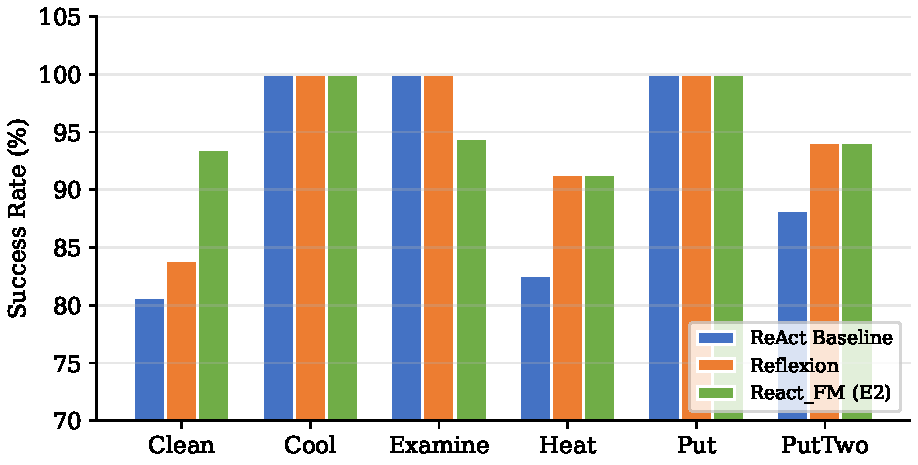
\includegraphics[width=\linewidth]{figures/alfworld_per_task.pdf}
    \caption{Per-task success rates on ALFWorld. \method{} shows the largest gains on \texttt{clean} (+12.8\%) and matches or exceeds Reflexion on all task types except \texttt{examine} (94.4\% vs 100\%).}
    \label{fig:per_task}
\end{figure}

\paragraph{Per-Task Analysis (ScienceWorld).}
Table~\ref{tab:sw_per_task} shows the per-task breakdown for the formal Step~4 protocol. Online \method{} does not dominate every task type. It clearly improves over the ReAct baseline on \texttt{melt} (+33.4 percentage points), \texttt{grow-plant} (+30.0), \texttt{power-component} (+40.0), and \texttt{use-thermometer} (+10.0), while the baseline remains stronger on \texttt{inclined-plane-friction-unnamed-surfaces}. ExpeL is strongest on several task types, especially \texttt{melt}, \texttt{lifespan-longest-lived-then-shortest-lived}, \texttt{test-conductivity}, and \texttt{use-thermometer}, but still fails on \texttt{mendelian-genetics-unknown-plant}. This heterogeneity matches the Step~4 runbook conclusion: memory helps on ScienceWorld, but the benefit is strongly task-dependent and unconditional intervention is not optimal.

\begin{table}[t]
\centering
\caption{Per-task success rates on the formal ScienceWorld Step~4 protocol.}
\label{tab:sw_per_task}
\small
\setlength{\tabcolsep}{3pt}
\begin{tabular}{p{3.5cm}ccccc}
\toprule
Task & Online & Offline & ReAct & Reflexion Adj & ExpeL \\
\midrule
boil & 33.3 & 33.3 & 44.4 & 11.1 & 44.4 \\
chemistry-mix & 37.5 & 37.5 & 25.0 & 25.0 & 37.5 \\
grow-plant & 30.0 & 30.0 & 0.0 & 30.0 & 50.0 \\
inclined-plane-friction-unnamed-surfaces & 40.0 & 50.0 & 60.0 & 50.0 & 30.0 \\
lifespan-longest-lived-then-shortest-lived & 50.0 & 60.0 & 50.0 & 40.0 & 70.0 \\
melt & 66.7 & 44.4 & 33.3 & 22.2 & 88.9 \\
mendelian-genetics-known-plant & 90.0 & 70.0 & 80.0 & 80.0 & 70.0 \\
mendelian-genetics-unknown-plant & 0.0 & 0.0 & 0.0 & 0.0 & 0.0 \\
power-component & 60.0 & 0.0 & 20.0 & 40.0 & 20.0 \\
test-conductivity & 10.0 & 10.0 & 20.0 & 30.0 & 40.0 \\
test-conductivity-of-unknown-substances & 0.0 & 20.0 & 30.0 & 20.0 & 30.0 \\
use-thermometer & 90.0 & 100.0 & 80.0 & 90.0 & 100.0 \\
\midrule
\textbf{Overall} & 41.44 & 39.64 & 37.84 & 36.94 & \textbf{49.55} \\
\bottomrule
\end{tabular}
\end{table}

\paragraph{WebShop Analysis.}
On WebShop, the primary failure modes are (1)~searching with overly specific queries that return few results, and (2)~selecting products without checking all required attributes (color, size, material). \method{} addresses these by storing failure-recovery pairs such as ``search with too many keywords failed $\to$ simplify search query'' and ``bought wrong color $\to$ check color option before buying.'' The progressive improvement from E1 to E2 (+4\% success rate, +0.031 average reward) demonstrates that these patterns transfer across shopping sessions with similar product categories.

\subsection{Learning Curve}
\label{sec:learning_curve}

\begin{figure}[t]
    \centering
    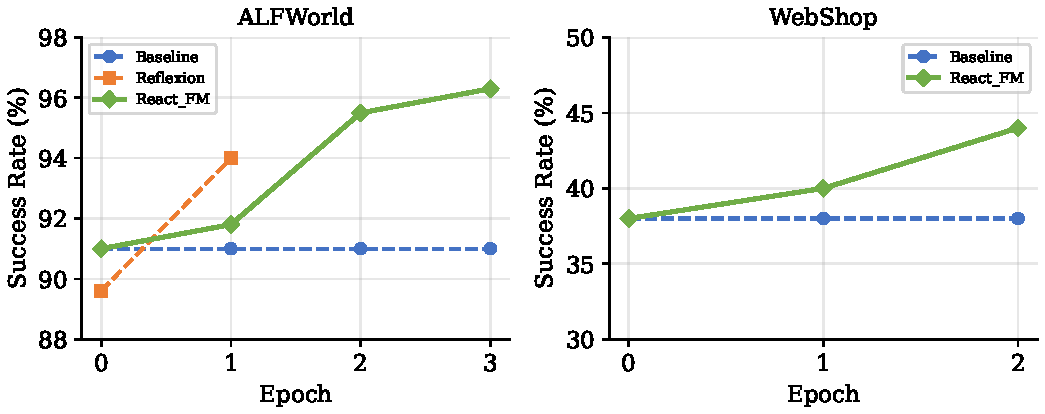
\includegraphics[width=\linewidth]{figures/learning_curve.pdf}
\caption{Success rate progression over epochs on ALFWorld and WebShop. \method{} shows consistent improvement as memory accumulates, while baselines remain flat. On ALFWorld (left), \method{} surpasses Reflexion at Epoch~2.}
\label{fig:learning_curve}
\end{figure}

Figure~\ref{fig:learning_curve} shows the learning curve on ALFWorld and WebShop, the two benchmarks where we have consistent multi-epoch curves under the same protocol. The pattern is consistent: \method{} improves with each epoch while baselines remain flat. On ALFWorld, \method{} improves from 91.8\% (E1) to 95.5\% (E2) to 96.3\% (E3), demonstrating that memory accumulation provides progressive benefit even beyond two epochs. On WebShop, E1 (40.0\%) to E2 (44.0\%) shows a +4\% improvement. On HotPotQA, EM improves from 0.395 (E1) to 0.430 (E2), and on ToolBench, pass rate improves from 62.1\% (E1) to 75.3\% (E2), both via skip-on-success carrying forward E1 successes while re-attempting failed instances with accumulated per-environment memory. ScienceWorld is not shown in Figure~\ref{fig:learning_curve} because the formal Step~4 result is reported under a dedicated one-pass no-gate protocol rather than the earlier pilot multi-epoch setting. Cross-environment memory sharing (\S\ref{sec:cross_env}) can further accelerate convergence on benchmarks with homogeneous task structures.

\subsection{Memory Analysis}
\label{sec:memory_analysis}

\begin{table}[t]
\centering
\caption{Memory statistics for \method{} on ALFWorld after Epoch~2.}
\label{tab:memory_stats}
\begin{tabular}{lcccccc}
\toprule
 & Clean & Cool & Examine & Heat & PutTwo & Put \\
\midrule
Entries & 16 & 9 & 53 & 15 & 11 & 6 \\
\bottomrule
\end{tabular}
\vspace{0.5em}

\begin{tabular}{lccc}
\toprule
Total Entries & Envs w/ Memory & Retrievals & Hits \\
\midrule
110 & 43/134 & 212 & 44 (20.8\%) \\
\bottomrule
\end{tabular}
\end{table}

Table~\ref{tab:memory_stats} reports memory statistics on ALFWorld. The system accumulated 110 failure-recovery entries across 43 environments (32\% of all environments experienced at least one detected failure). \texttt{Examine} tasks generated the most entries (53), consistent with their complex multi-step nature. The retrieval hit rate of 20.8\% (44 out of 212 queries) indicates selective retrieval---memories are injected only when relevant matches exist, avoiding noise injection.

\paragraph{Token Efficiency.} On WebShop, \method{} E2 uses 3.89M tokens compared to the baseline's 3.83M (+1.6\%), achieving a +6\% success improvement for minimal token overhead. On the formal ScienceWorld Step~4 protocol, online \method{} uses 197.2K tokens per episode versus 185.5K for the baseline (+6.3\%) while improving success by +3.60 percentage points and average raw score by +17.04. Offline memory is slightly cheaper at 180.4K tokens per episode, while corrected Reflexion only appears cheaper under selected-output accounting; its true runtime lower bound is 212.6K tokens per episode because both passes are executed. The judge LLM adds 82K tokens on ALFWorld (4.7\% of agent tokens), and the extractor adds 24K (1.4\%), confirming that the failure detection and extraction components are lightweight.

\paragraph{Failure Detection Analysis.} Table~\ref{tab:detection_stats} summarizes failure detection on the benchmarks where the final protocol uses the implicit failure judge. On ALFWorld, all 56 detected failures were \emph{explicit} (``Nothing happens''), detected via zero-cost pattern matching with no LLM judge invocations---the detection mechanism is fully deterministic. On WebShop, 49\% of episodes trigger at least one failure detection, and the implicit judge accounts for 94K tokens. The formal ScienceWorld Step~4 protocol disables implicit judge-based detection in favor of explicit rules, so we do not report ScienceWorld judge-token statistics in the main paper.

\paragraph{Judge Precision Audit.} To validate the implicit failure judge, we manually audited a sample of judge-triggered detections (``unproductive'' type) from Epoch~2 on WebShop. We examined 30 unique (action, observation) pairs: all 30 were true positives---search queries returning the instruction page without navigating to product results, correctly flagged as unproductive (precision: 100\%). We do not report a corresponding ScienceWorld audit in the main paper because the final ScienceWorld Step~4 protocol no longer uses judge-based implicit detection.

\paragraph{Recall Limitations.} Our audit measures precision (fraction of detections that are true failures) but not recall (fraction of true failures that are detected). Estimating recall would require labeling all action-observation pairs in a set of episodes, not just those flagged by the judge---a substantially more expensive annotation effort. We note two mitigating factors: (1)~explicit failure detection via pattern matching is deterministic and has near-perfect recall for its covered failure types (e.g., ``Nothing happens'' in ALFWorld); (2)~the E1$\to$E2 improvement on all benchmarks provides indirect evidence that the detector captures a meaningful fraction of failures, since missed failures cannot contribute to memory accumulation. A comprehensive recall evaluation with multiple annotators is an important direction for future work.

\begin{table}[h]
\centering
\caption{Failure detection statistics for the judge-enabled final protocols (Epoch~2).}
\label{tab:detection_stats}
\small
\begin{tabular}{lccccc}
\toprule
Benchmark & Episodes w/ failures & Total detections & Judge tokens & Explicit only? \\
\midrule
ALFWorld & 9/134 (6.7\%) & 56 & 0 & Yes \\
WebShop & 49/100 (49.0\%) & 567 & 94K & No \\
\bottomrule
\end{tabular}
\end{table}

\subsection{Ablation Studies}
\label{sec:ablation}

We design ablation experiments to isolate the contributions of \method{}'s two key design choices: (1)~\emph{when} to inject memories (retrieval timing), and (2)~\emph{what} to store (memory format). Timing and detection ablations are evaluated on ALFWorld and WebShop. ScienceWorld is analyzed through the dedicated Step~4 comparison in Table~\ref{tab:sw_step4}, because the final formal protocol differs from the earlier pilot multi-epoch ablations.

\paragraph{Ablation 1: Retrieval Timing.}
We compare injection modes while keeping the memory format fixed (failure-recovery pairs). Table~\ref{tab:ablation_timing} reports ALFWorld and WebShop.

\begin{table}[h]
\centering
\caption{Ablation on retrieval timing (Epoch~2). All variants use the same failure-recovery memory format.}
\label{tab:ablation_timing}
\small
\begin{tabular}{lccc}
\toprule
\multirow{2}{*}{Injection Mode} & \multicolumn{2}{c}{ALFWorld} & WebShop \\
\cmidrule(lr){2-3} \cmidrule(lr){4-4}
 & E1 & E2 & E2 \\
\midrule
No memory (baseline) & 91.0\% & --- & 38.0\% \\
Episode-level & 90.2\% & 94.8\% & 45.0\% \\
\textbf{In-loop (ours)} & \textbf{91.8\%} & \textbf{95.5\%} & 44.0\% \\
\bottomrule
\end{tabular}
\end{table}

\paragraph{Ablation 2: Memory Format.}
We compare three memory storage formats while keeping the injection mode fixed (in-loop). Table~\ref{tab:ablation_format} extends this ablation to ALFWorld and WebShop.

\begin{table}[h]
\centering
\caption{Ablation on memory format (Epoch~2). All variants use in-loop injection timing.}
\label{tab:ablation_format}
\small
\begin{tabular}{lp{3.5cm}cccc}
\toprule
\multirow{2}{*}{Memory Format} & \multirow{2}{*}{What is stored} & \multicolumn{2}{c}{ALFWorld} & \multicolumn{2}{c}{WebShop} \\
\cmidrule(lr){3-4} \cmidrule(lr){5-6}
 & & E1 & E2 & E2 SR & E2 Rew \\
\midrule
Success trajectory & Key steps from successful episodes & 91.8\% & 94.8\% & 48.0\% & .456 \\
Reflexion reflection & Free-text reflections on failures & 89.6\% & 91.8\% & 46.5\% & .449 \\
\textbf{Failure-recovery (ours)} & (failed action, observation, fix) & \textbf{91.8\%} & \textbf{95.5\%} & 44.0\% & .416 \\
\bottomrule
\end{tabular}
\end{table}

\paragraph{Ablation 3: Detection vs.\ Retrieval.}
To isolate the contribution of failure detection from memory retrieval, we run a \emph{detection-only} control (\texttt{inject\_mode=none}): the failure detector is active but retrieved memories are never injected. We evaluate this on ALFWorld and WebShop.

\begin{table}[h]
\centering
\caption{Detection-only control (Epoch~2 full-set metrics). Detection-only activates the failure detector but disables memory injection.}
\label{tab:detection_only}
\small
\begin{tabular}{lcc}
\toprule
System & ALFWorld & WebShop \\
\midrule
ReAct Baseline & 91.0\% & 38.0\% \\
Detection-only (E2) & 93.3\% & 42.0\% \\
\textbf{\method{} full (E2)} & \textbf{95.5\%} & \textbf{44.0\%} \\
\bottomrule
\end{tabular}
\end{table}

On ALFWorld, detection-only (93.3\%) improves over the baseline (91.0\%) but falls short of the full system (95.5\%), confirming that memory retrieval provides an additional +2.2\% beyond detection alone. On WebShop, detection-only (42.0\%) and the full system (44.0\%) both improve over the baseline, with a small gap suggesting retrieval provides modest additional benefit.

\paragraph{Ablation 4: Retrieval Method.}
We compare three retrieval methods while keeping all other components fixed (in-loop injection, failure-recovery format). Table~\ref{tab:retrieval_ablation} presents results on ALFWorld and WebShop.

\begin{table}[h]
\centering
\caption{Retrieval method ablation (Epoch~2). WebShop results are from a partial run (70/100 environments) due to API availability.}
\label{tab:retrieval_ablation}
\small
\begin{tabular}{lccc}
\toprule
\multirow{2}{*}{Retrieval Method} & ALFWorld & \multicolumn{2}{c}{WebShop$^*$} \\
\cmidrule(lr){2-2} \cmidrule(lr){3-4}
 & E2 & E2 SR & E2 Rew \\
\midrule
BM25-only & 95.5\% & 41.4\% & .396 \\
Embedding-only & 93.1\% & 40.0\% & .403 \\
\textbf{Hybrid RRF (ours)} & \textbf{95.5\%} & \textbf{44.0\%} & \textbf{.416} \\
\bottomrule
\multicolumn{4}{l}{\footnotesize $^*$WebShop: 70/100 environments completed.}
\end{tabular}
\end{table}

On ALFWorld, hybrid RRF (95.5\%) matches BM25-only (95.5\%) and outperforms embedding-only (93.1\%). The strong BM25 performance reflects ALFWorld's constrained vocabulary where lexical matching is highly effective. On WebShop (partial results, 70/100 environments), hybrid RRF (44.0\%) outperforms both BM25-only (41.4\%) and embedding-only (40.0\%), suggesting that the hybrid approach provides more benefit when tasks involve diverse natural language descriptions. Embedding-only retrieval underperforms on both benchmarks, likely because semantic similarity is less discriminative when failure descriptions share similar language patterns.

\textbf{Retrieval timing} (Table~\ref{tab:ablation_timing}): The cross-benchmark results reveal that the advantage of in-loop over episode-level injection is \emph{conditional on task structure}. On ALFWorld, in-loop injection (95.5\%) shows a small gain over episode-level (94.8\%, $p{=}0.415$)---directional but not significant. On WebShop, episode-level (45.0\%) slightly outperforms in-loop (44.0\%), suggesting that for short-horizon tasks, upfront guidance may suffice. The formal ScienceWorld Step~4 comparison in Table~\ref{tab:sw_step4} is consistent with the usefulness of online in-loop memory, but because it also changes the memory source and evaluation protocol, we do not interpret it as a clean timing-only ablation. Our claim is therefore conditional rather than universal: failure-triggered in-loop retrieval appears most valuable when tasks are long-horizon and action failures are varied enough that fixed upfront guidance is brittle.

\textbf{Memory format} (Table~\ref{tab:ablation_format}): On ALFWorld, failure-recovery pairs (95.5\%) outperform success trajectories (94.8\%, $p{=}0.428$) and Reflexion-style reflections (91.8\%, $p{=}0.056$). Interestingly, on WebShop the pattern reverses: success trajectories (48.0\%) and Reflexion reflections (46.5\%) both outperform failure-recovery pairs (44.0\%). This suggests that for short-horizon shopping tasks with uniform structure, higher-level guidance (what worked or what to avoid) may be more transferable than specific failure-recovery sequences. The ALFWorld advantage of failure-recovery pairs over abstract reflections (+3.7\%, $p{=}0.056$) remains the largest observed effect, consistent with the hypothesis that structured, actionable memories are most valuable for long-horizon tasks with diverse failure modes.

\subsection{Qualitative Examples}
\label{sec:qualitative}

Table~\ref{tab:examples} shows representative failure-recovery pairs extracted by \method{} on ALFWorld. These examples illustrate three common failure patterns: (1)~interacting with closed containers without opening them first, (2)~attempting actions from the wrong location, and (3)~using incorrect receptacles. In each case, the stored solution provides a concrete, directly executable corrective sequence rather than an abstract rule.

\begin{table}[t]
\centering
\caption{Representative failure-recovery pairs from \method{}'s memory store (ALFWorld).}
\label{tab:examples}
\small
\begin{tabular}{p{1.2cm}p{3.0cm}p{3.0cm}}
\toprule
Type & Failed Action $\to$ Obs & Stored Solution \\
\midrule
cool & \texttt{put tomato in microwave} $\to$ ``Nothing happens'' & \texttt{open microwave} $\to$ \texttt{put tomato in microwave} \\
\addlinespace
examine & \texttt{open drawer 2} $\to$ ``Nothing happens'' & \texttt{go to drawer 2} $\to$ \texttt{open drawer 2} \\
\addlinespace
clean & \texttt{clean towel with sink} $\to$ ``Nothing happens'' & \texttt{put towel in sink} $\to$ \texttt{clean towel with sink} \\
\bottomrule
\end{tabular}
\end{table}

\subsection{Cross-Benchmark Discussion}
\label{sec:discussion}

The five benchmarks test \method{} under diverse conditions, and the mixed results suggest an \emph{operating regime hypothesis} for failure-triggered in-loop memory. Table~\ref{tab:regime} summarizes the key characteristics. We emphasize that this regime analysis is exploratory---based on correlations across five benchmarks with confounds (different backbones, task structures)---rather than a rigorously demonstrated operating law.

\begin{table}[h]
\centering
\caption{Exploratory operating-regime analysis. \method{} is strongest on ALFWorld and achieves the highest raw score on the formal ScienceWorld Step~4 no-gate protocol, while ExpeL achieves the highest ScienceWorld success rate. $\Delta$ = \method{} gain over the corresponding baseline metric.}
\label{tab:regime}
\small
\setlength{\tabcolsep}{2pt}
\resizebox{\linewidth}{!}{%
\begin{tabular}{lcccl}
\toprule
Benchmark & Max Steps & Dominant Failure & $\Delta$ & Best Method \\
\midrule
ScienceWorld & 100 & Action-level, task-dependent & +3.60 pp succ.; +17.04 score & ExpeL (succ.) / \method{} (score) \\
ALFWorld & 50 & Action-level & +4.5 pp succ. & \method{} \\
ToolBench & 12 & External (API) & +12.5 pp pass & ExpeL \\
WebShop & 15 & Mixed / short-horizon & +6.0 pp succ. & ExpeL \\
HotPotQA & 8 & Strategic & +3.4 pp EM & ExpeL \\
\bottomrule
\end{tabular}
}
\end{table}

\method{} achieves the strongest result on ALFWorld and the highest raw score on the formal ScienceWorld Step~4 no-gate protocol. On ALFWorld, the margin over ExpeL and Reflexion is not significant, but the system still achieves the top success rate without restarts or cross-trajectory comparison. On ScienceWorld, online \method{} improves over the baseline in both success rate (+3.60 percentage points) and raw score (+17.04), indicating better partial progress even when episodes do not reach 100. ExpeL achieves the highest Step~4 success rate after first collecting a full epoch of trajectories, while \method{} retains the highest raw score and learns online within the test stream. On benchmarks where the dominant failure mode is \emph{strategic} (HotPotQA) or \emph{external} (ToolBench, API cache misses), offline methods like ExpeL achieve higher overall performance by extracting abstract strategies. ToolBench is instructive: \method{} achieves a large gain over the baseline (+12.5\%) but still ranks third because the dominant failure mode requires strategic adaptation rather than action-level correction. We therefore view \method{} as \emph{complementary} to episode-level methods: in-loop correction addresses recoverable action failures, while episode-level reflection is better suited to strategic failures.

\paragraph{Online vs.\ Offline Learning.} A key architectural advantage of \method{} is its \emph{online} learning paradigm. Memories extracted after each episode are immediately available to subsequent environments within the same epoch. In contrast, ExpeL requires a complete first epoch to collect trajectories before batch-extracting insights for Epoch~2, and Reflexion requires two trials per environment. ScienceWorld Step~4 makes this distinction concrete: online \method{} starts with an empty memory and still outperforms the offline-memory variant that begins test-time evaluation with a pre-collected train-memory bank. ExpeL is stronger in final success after a full collection epoch, but this requires completing Epoch~1 before the extracted insights can help. Thus \method{} is advantageous when tasks arrive as a stream and a ``collect first, learn later'' approach is impractical.

\paragraph{Cross-Benchmark Caveats.} We note that direct cross-benchmark comparisons should be interpreted with caution due to two confounds: (1)~different LLM backbones are used across benchmarks (Qwen3.5-9B for ALFWorld/WebShop, DeepSeek-V3.2 for ScienceWorld/HotPotQA/ToolBench), and (2)~benchmark difficulty and failure mode distributions vary widely. Within each benchmark, all systems use the same backbone, prompt, and budget, so within-benchmark comparisons are controlled. The regime analysis in Table~\ref{tab:regime} should be read as identifying \emph{which task characteristics favor in-loop memory} rather than claiming general superiority across all settings.

\paragraph{Source of Gains.} The detection-only control (Table~\ref{tab:detection_only}) provides the clearest evidence for disentangling detection from retrieval contributions on ALFWorld and WebShop. On ALFWorld (+2.2\% over detection-only), retrieval provides a modest but consistent boost; on WebShop (+2.0\%), the gap is similar. ScienceWorld Step~4 exposes a different effect: online in-loop adaptation outperforms loading an offline memory bank collected on train (41.44\% vs.\ 39.64\%), suggesting that fresh within-protocol experience matters on harder scientific tasks.

\paragraph{Memory Utilization and Adaptation Dynamics.} Across the multi-epoch benchmarks, E2 recovers environments that E1 failed on (5 on ALFWorld, 4 on WebShop). On HotPotQA and ToolBench, the per-environment isolation means E2 retrieves the same memories as E1, yielding no additional improvement---cross-environment memory sharing addresses this limitation on HotPotQA (+1.3\% EM in one epoch) but causes negative transfer on ToolBench ($-$19.9\%) due to API heterogeneity (\S\ref{sec:cross_env}). On ALFWorld, 42 of 134 environments (31\%) accumulate memory entries after E1; on WebShop, 74 of 100 (74\%). On the formal ScienceWorld Step~4 run, the single online pass stores 297 memories and records 1,049 retrieval hits from 1,293 retrieval attempts, indicating that memory is heavily exercised even without repeated epochs.

\subsection{Cross-Environment Memory Transfer}
\label{sec:cross_env}

A key limitation of per-environment memory isolation is that experiences from one environment cannot help in others, even when failure patterns are shared. To test whether \emph{within-benchmark cross-environment transfer} is viable, we run a \emph{shared-memory} variant where all environments contribute to and retrieve from a single global memory store (filtered by task type), rather than maintaining isolated per-environment memories. We evaluate this on three benchmarks---WebShop, HotPotQA, and ToolBench---which vary widely in task homogeneity. This tests transfer within recurring task families, not broad out-of-distribution generalization.

\begin{table}[h]
\centering
\caption{Cross-environment memory transfer across three benchmarks (single epoch). Shared memory pools failure-recovery entries from all environments, filtered by task type. $\Delta$ vs.\ Per-env E1 shows the effect of cross-environment sharing within one epoch.}
\label{tab:cross_env}
\small
\begin{tabular}{llcccc}
\toprule
Benchmark & Configuration & Epochs & Metric & Hit Rate \\
\midrule
\multirow{3}{*}{WebShop} & Per-env E1 & 1 & 40.0\% / .385 & 0\% \\
 & Per-env E2 & 2 & 44.0\% / .416 & 27\% \\
 & \textbf{Shared E1} & \textbf{1} & \textbf{44.0\% / .423} & \textbf{98\%} \\
\midrule
\multirow{3}{*}{HotPotQA} & Per-env E1 & 1 & .395 / .489 & --- \\
 & Per-env E2 & 2 & .430 / .515 & --- \\
 & \textbf{Shared E1} & \textbf{1} & \textbf{.408 / .504} & \textbf{99\%} \\
\midrule
\multirow{3}{*}{ToolBench} & Per-env E1 & 1 & 62.1\% & 0\% \\
 & Per-env E2 & 2 & 75.3\% & --- \\
 & Shared E1 & 1 & 42.2\% & 98\% \\
\bottomrule
\end{tabular}
\vspace{0.3em}

{\footnotesize WebShop metric: Succ.\,/\,Reward. HotPotQA metric: EM\,/\,F1. ToolBench metric: Pass rate.}
\end{table}

Table~\ref{tab:cross_env} reveals that the effectiveness of cross-environment memory sharing depends critically on \emph{task homogeneity}---the degree to which different environments share similar failure patterns.

\paragraph{WebShop (positive transfer).} Shared-memory \method{} achieves 44.0\% success rate in a single epoch---matching the per-environment E2 result that requires two epochs. The retrieval hit rate jumps from 0\% (per-env E1, no prior memories) to 98\% (shared, memories from earlier environments are available). All WebShop sessions involve the same task structure (search $\to$ browse $\to$ select $\to$ buy), so failure patterns such as ``simplify search queries'' and ``check color options before buying'' transfer effectively across sessions.

\paragraph{HotPotQA (moderate transfer).} Shared memory improves EM from 0.395 (per-env E1) to 0.408 (+1.3\%) in a single epoch, with F1 improving from 0.489 to 0.504. This is a meaningful improvement but falls short of per-env E2 (EM=0.430), which benefits from retrying the \emph{same} question with its own failure memory. HotPotQA questions share some procedural patterns (e.g., search strategies, disambiguation tactics) but differ in domain-specific knowledge, limiting cross-question transfer.

\paragraph{ToolBench (negative transfer).} Cross-environment sharing \emph{hurts} performance: pass rate drops from 62.1\% (per-env E1) to 42.2\% ($-$19.9\%), well below the baseline (62.8\%). The decline is uniform across all subsets ($-$12\% to $-$27\%). ToolBench tasks use diverse APIs with distinct parameter schemas and error modes; failure-recovery pairs from one API (e.g., weather data) are irrelevant or misleading when injected into another (e.g., financial data). Despite task-type filtering (memories are restricted to the same G1/G2/G3 subset), the heterogeneity within each subset is too high for meaningful transfer.

\paragraph{Task Homogeneity as a Predictor.} These results suggest a simple predictor for when cross-environment sharing helps: \emph{the more homogeneous the task structure within a benchmark, the more beneficial shared memory}. WebShop (single task structure) $\to$ strong positive transfer. HotPotQA (shared procedure, diverse content) $\to$ moderate transfer. ToolBench (diverse APIs with distinct schemas) $\to$ negative transfer. This finding has practical implications: cross-environment sharing should be enabled selectively based on task similarity, rather than applied universally. A natural extension is to cluster environments by similarity and share memory only within clusters, which we leave to future work.
